% !TeX program = lualatex
\documentclass[../skript/main.tex]{subfiles}

\begin{document}\label{chap:hardwarearchitektur}
\chapter{Hardwarearchitektur}

\section{Worum geht es?}
Unter \textbf{Hardwarearchitektur} versteht man den grundsätzlichen Aufbau eines Rechners:
Welche Bausteine gibt es (z.\,B.\ Prozessor, Speicher, Ein-/Ausgabe), wie sind sie
\emph{organisiert} und \emph{verbunden}, und wie arbeiten sie zusammen, um Programme auszuführen?
Die heute dominierende Grundidee ist die \textbf{von-Neumann-Architektur}.

\section{John von Neumann und die Grundidee}
In den 1940er Jahren formulierte John von Neumann (gemeinsam mit weiteren Pionieren um ENIAC/EDVAC)
eine einfache, aber revolutionäre Idee: \textbf{Programm und Daten liegen im gleichen Speicher.}
Das heißt, ein Programm ist selbst nur eine Folge von Zahlen (Maschinenbefehlen), die genau wie Daten
im Hauptspeicher abgelegt und von der CPU geholt werden. Diese \emph{Stored-Program}-Idee macht
Rechner \emph{flexibel} (beliebige Programme ladbar) und \emph{universell}.



% (Optionaler Hinweis, falls du ihn setzen möchtest:)
%\paragraph{Hinweis.} Moderne Prozessoren mildern den Engpass z.\,B. durch schnelle \emph{Caches} in der CPU, 
%Vorabruf (Prefetch) und parallele Arbeitsschritte (Pipelining). Das Grundproblem — ein gemeinsamer Weg 
%für Befehle und Daten — bleibt dabei aber die Ursache des Flaschenhalses.


\subsection*{Bausteine im von-Neumann-Modell}
\begin{itemize}
	\item \textbf{CPU (Prozessor)} mit
	\begin{itemize}
		\item \textbf{Steuerwerk} (kontrolliert den Ablauf, interpretiert Befehle),
		\item \textbf{Rechenwerk/ALU} (führt Operationen wie Addieren, Vergleichen aus),
		\item \textbf{Registern} (kleinste, sehr schnelle Speicherplätze, z.\,B.\ Akkumulator, Program Counter).
	\end{itemize}
	\item \textbf{Hauptspeicher (RAM)}: enthält \emph{sowohl} Daten \emph{als auch} Befehle.
	\item \textbf{Ein-/Ausgabe (I/O)}: Tastatur, Bildschirm, Netz, Sensoren, Aktoren \dots
	\item \textbf{Bus-System}: Verbindet die Bausteine (Adress-, Daten- und Steuerbus).
\end{itemize}

\begin{figure}[H]
	\centering
	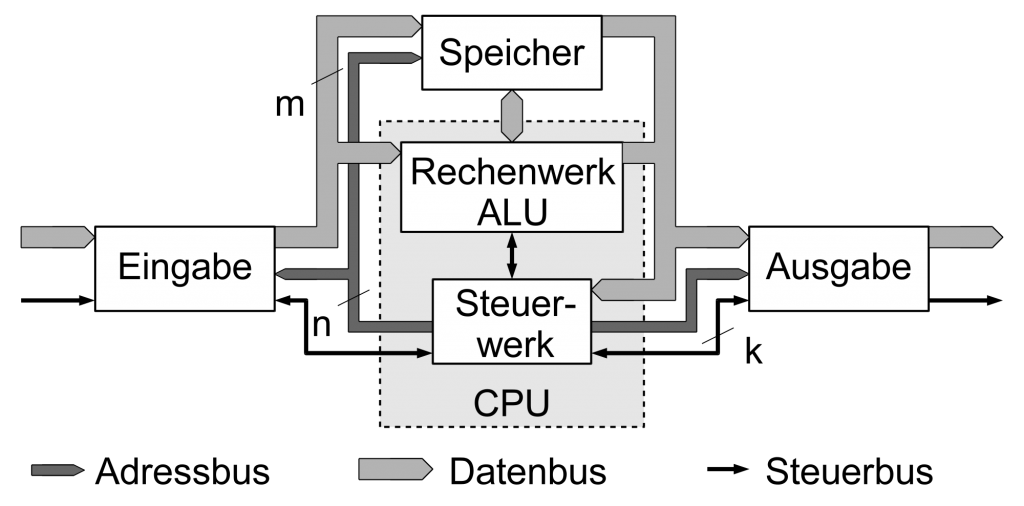
\includegraphics[width=.75\textwidth]{vonNeumannarchitektur.png}
	\caption{Architektur von Neumann Rechners.}
	\label{fig:vonNeumannarchitektur}
\end{figure}

Im Von-Neumann-Rechner steckt die „Denkarbeit“ in der CPU. Sie besteht aus zwei Hauptteilen: dem Rechenwerk (ALU), das z. B. addiert, vergleicht und logisch verknüpft, und dem Steuerwerk, das den Ablauf organisiert. Die CPU arbeitet Befehle nacheinander ab: Sie holt einen Befehl aus dem Speicher (Fetch), versteht ihn (Decode) und führt ihn aus (Execute). Sowohl Befehle als auch die dazugehörigen Daten werden aus demselben Arbeitsspeicher geholt.\\
Damit CPU, Speicher und Ein-/Ausgabegeräte miteinander sprechen können, gibt es gemeinsame Leitungen, das Bus-System. Über den Adressbus wird gesagt, „wo“ etwas liegt, über den Datenbus „was“ übertragen wird, und der Steuerbus regelt das „wie“ (Lesen/Schreiben, Takt, Signale).\\
Weil Befehle und Daten denselben Weg benutzen entsteht in dem Prozess der sogenannte Von-Neumann-Flaschenhals. Auf Grund der Tatsache, dass zur gleichen Zeit neue Befehle geholt und Daten gelesen oder geschrieben werden, kommt es zu Staus auf dem Bus: Die CPU könnte weiterrechnen, muss aber warten, bis der Bus wieder frei ist.\\ \\
Alltagsbild: Stell dir eine Straße mit nur einer Spur vor. Darauf fahren sowohl „Befehls-Autos“ als auch „Daten-Laster“. Wenn viele Daten unterwegs sind, stehen die Befehle im Stau – die CPU wartet.

Kleines Beispiel: Die drei Befehle „LOAD A“, „ADD B“, „STORE A“.

\begin{enumerate}
	\item LOAD A: Die CPU holt den Befehl, versteht ihn und fordert die Daten an Adresse A an. Während die Daten geladen werden, ist der Bus belegt.
	\item Die CPU würde gern sofort den nächsten Befehl (ADD B) holen, kann aber nicht, weil der Bus noch mit dem Datentransfer für LOAD beschäftigt ist. Es entsteht ein Wartetakt.
	\item Sobald die Daten aus A angekommen sind, kann die CPU weiterarbeiten: Sie holt nun den ADD-Befehl, liest die Daten von B und rechnet.
	\item STORE A schreibt das Ergebnis zurück in den Speicher – wieder wird der Bus belegt.
\end{enumerate}





%\begin{figure}[H]
%	\centering
%	\setlength{\fboxsep}{6pt}
%	\begin{tabular}{c}
%		\fbox{\parbox{0.8\textwidth}{\centering Ein-/Ausgabe (I/O)}}\\[0.5em]
%		$\updownarrow$ \emph{Bus-System} \\[0.5em]
%		\fbox{\parbox{0.8\textwidth}{\centering Hauptspeicher (Programme \& Daten)}}\\[0.5em]
%		$\updownarrow$ \emph{Bus-System} \\[0.5em]
%		\fbox{\parbox{0.8\textwidth}{\centering CPU = Steuerwerk + ALU + Register}}
%	\end{tabular}
%	\caption{Vereinfachtes von-Neumann-Modell.}
%\end{figure}

\section{Der Befehlszyklus (Fetch–Decode–Execute)}
Jeder Maschinenbefehl läuft in drei Schritten durch die CPU:
\begin{enumerate}
	\item \textbf{Fetch} (Holen): Der \emph{Program Counter (PC)} zeigt auf die nächste Befehlsadresse.
	Der Befehl wird aus dem Speicher gelesen und in das \emph{Befehlsregister (IR)} gelegt.
	\item \textbf{Decode} (Dekodieren): Das Steuerwerk „versteht“, welcher Operationstyp gemeint ist
	(z.\,B.\ ADD, LOAD, STORE) und welche Operanden/Adressen beteiligt sind.
	\item \textbf{Execute} (Ausführen): Die ALU rechnet bzw.\ I/O/Speicherzugriffe passieren.
	Der PC wird auf den nächsten Befehl gesetzt (oder bei Sprüngen angepasst).
\end{enumerate}

\paragraph{Mini-Beispiel (gedankliches Maschinenprogramm).}
\begin{lstlisting}[caption={Addition zweier Speicherstellen und Ablage des Ergebnisses}]
	LOAD R0, [x]   ; lade x in Register R0
	LOAD R1, [y]   ; lade y in Register R1
	ADD  R0, R1    ; R0 := R0 + R1
	STORE R0, [z]  ; speichere Ergebnis in z
\end{lstlisting}
Hier holt die CPU nacheinander die Befehle (Fetch), dekodiert sie (Decode) und führt sie aus (Execute).

%\section{Speicher, Wortbreite und Adressierung}
%\begin{itemize}
%	\item \textbf{Wortbreite} (z.\,B.\ 32 Bit, 64 Bit) gibt an, wie viele Bits die CPU in einem Schritt besonders effizient verarbeitet
%	(Register- und ALU-Breite). Sie beeinflusst u.\,a.\ den darstellbaren Adressraum und Zahlenbereich.
%	\item \textbf{Adressbus/Datenbus}: Mit \(n\) Adressleitungen kann man \(2^n\) Speicheradressen ansprechen.
%	\item \textbf{Speicherhierarchie}: Register \(\rightarrow\) Caches (L1/L2/L3) \(\rightarrow\) RAM \(\rightarrow\) SSD/HDD.
%	Je näher an der CPU, desto schneller (aber kleiner/teurer).
%\end{itemize}

\section{Warum ist das so erfolgreich?}
\begin{itemize}
	\item \textbf{Einfachheit}: Ein einheitlicher Speicher für Programme und Daten macht die Hardware und das Laden von Programmen einfach.
	\item \textbf{Flexibilität}: Beliebige Programme können nachgeladen werden; Selbstmodifizierender Code ist (theoretisch) möglich.
	\item \textbf{Universalität}: Mit genug Speicher und Zeit kann ein solcher Rechner jede berechenbare Aufgabe lösen (Church–Turing-Idee).
\end{itemize}

% Abschnitt für dein Skript (schülergerecht zusammengeführt und gestrafft)

\section{Grenzen: der Von-Neumann-Flaschenhals}
Im klassischen Von-Neumann-Modell teilen sich \emph{Programmcode} (Befehle) und \emph{Daten}
denselben Speicher und denselben Bus. Beide benutzen also die gleiche „Datenstraße“.
Dadurch konkurrieren sie um Bandbreite: Die CPU könnte weiterrechnen, muss aber oft warten,
bis neue Befehle \emph{oder} Daten geliefert werden. Diesen Engpass nennt man den
\textbf{Von-Neumann-Flaschenhals}.

\paragraph{Kurz gefragt: Was hilft grundsätzlich?}
\begin{itemize}
	\item \textbf{Nähere Vorräte:} \emph{Caches} (kleine, sehr schnelle Zwischenspeicher in der CPU).
	\item \textbf{Früher holen:} \emph{Prefetch} (Daten/Befehle im Voraus anfordern).
	\item \textbf{Mehr gleichzeitig:} \emph{Pipeline}, \emph{Superskalarität}, \emph{Multi-Core}, \emph{Vektor/SIMD}.
	\item \textbf{Breitere/schnellere Wege:} schnellere Speichertechniken, breitere Busse.
\end{itemize}

\begin{quote}\small
	\textbf{Merksatz:} Wenn die CPU warten muss, helfen \emph{nähere Vorräte}, \emph{rechtzeitig holen},
	\emph{gleichzeitig arbeiten} und \emph{breitere/schnellere Verbindungen}.
\end{quote}

\section{Harvard vs.\ Von Neumann (und was man heute wirklich baut)}
Die \textbf{Harvard-Architektur} trennt \emph{Befehls-} und \emph{Datenspeicher} (je ein eigener Bus).
Vorteil: Code und Daten können \emph{gleichzeitig} geholt werden – der Engpass an dieser Stelle entfällt.
Viele Mikrocontroller/DSPs arbeiten so.

In PCs und Laptops nutzt man meist ein \emph{hybrides} Vorgehen:
Moderne CPUs bleiben vom Speicherbild her \emph{Von Neumann} (ein gemeinsamer Hauptspeicher),
verwenden aber direkt an der CPU getrennte \textbf{Instruktions-} und \textbf{Daten-Caches}
(\emph{Modified Harvard} auf Cache-Ebene). So verbindet man die
\emph{Programmierfreundlichkeit} des Von-Neumann-Modells mit Leistungsgewinnen durch getrennte, nahe Wege.

\section{Erweiterte Von-Neumann-Rechner: die wichtigsten Ideen}
In der Praxis ist die CPU oft schneller als der Weg zu den Daten. Deshalb hat man das Grundmodell
\emph{weiterentwickelt} (keine völlig neue Architektur, sondern Ergänzungen):

\subsection*{1) Speicherhierarchie und Caches}
Statt immer den vergleichsweise langsamen Hauptspeicher zu fragen, nutzt die CPU kleine,
extrem schnelle \textbf{Caches} direkt am Kern:
L1 (sehr klein, sehr schnell), dahinter L2/L3 (größer, etwas langsamer).
Häufig gebrauchte Befehle und Daten liegen dann „um die Ecke“.
Viele CPUs trennen den L1 in \textbf{I-Cache} (Instruktionen) und \textbf{D-Cache} (Daten),
sodass Code \emph{und} Daten parallel kommen.

\subsection*{2) Vorabruf und Vorhersage}
Die CPU versucht zu erraten, was sie als Nächstes braucht:
\emph{Prefetch} holt Daten/Befehle im Voraus.
\emph{Sprungvorhersage} (Branch Prediction) rät den nächsten Programmpfad.
Treffen die Vorhersagen, spart das viele Takte; liegen sie daneben, wird zurückgerollt.

\subsection*{3) Fließbandarbeit: Pipelining und Superskalarität}
Befehle werden in Stufen zerlegt (z.\,B.\ Fetch, Decode, Execute, Writeback).
Mehrere Befehle können gleichzeitig in \emph{verschiedenen} Stufen sein (\textbf{Pipeline}).
\textbf{Superskalarität} startet sogar \emph{mehr als einen} Befehl pro Takt, wenn Einheiten frei sind.

\subsection*{4) Keine Zeit verlieren: Out-of-Order}
Muss ein Befehl warten (z.\,B.\ auf Daten), arbeitet die CPU mit einem anderen, unabhängigen
Befehl weiter. So bleiben Recheneinheiten ausgelastet und Wartezeiten fallen weniger ins Gewicht.

\subsection*{5) Schnellere und breitere Verbindungen}
„Die Straßen wurden ausgebaut“: breitere Datenpfade, schnellere Speicher (z.\,B.\ moderne DDR-/HBM-Verfahren),
intelligente Speichercontroller und \emph{DMA} (Direct Memory Access), damit Daten bewegt werden können,
ohne die CPU zu blockieren.

\subsection*{6) Mehr Parallelität: Multi-Core und Vektor/SIMD}
Statt nur einem Kern rechnen \textbf{mehrere Kerne} gleichzeitig an verschiedenen Aufgaben.
\textbf{Vektor-/SIMD-Einheiten} wenden \emph{eine} Operation auf \emph{viele} Daten gleichzeitig an
(z.\,B.\ bei Bild-/Audioverarbeitung).

\paragraph{Wichtig zu wissen.}
All diese Maßnahmen \emph{mildern} den Von-Neumann-Flaschenhals deutlich, beseitigen ihn aber nicht ganz.
Wenn Daten nicht im Cache sind oder Programme sehr sprunghaft arbeiten, muss die CPU weiterhin warten.
Moderne Rechner sind daher ein Mix aus \emph{schlauem Vorrat} (Caches), \emph{Vorausschau}
(Prefetch/Prediction), \emph{Parallelität} (Pipeline, Multi-Core, SIMD) und \emph{breiteren/schnelleren Wegen},
damit aus „Warten auf Daten“ so oft wie möglich „Rechnen“ wird.


	
\end{document}